% answers.tex —— 1977 年·黑龙江卷 · 参考答案与详细解析片段
% 由 tools/generate_projects.py 依来源总账自 1977/1977_数学真题_黑龙江_试题.md + 1977/1977_数学真题_黑龙江_解析正文.md + 1977/1977_数学真题_黑龙江_答案要点.md 生成，勿手改（改源 MD 后重跑）


\begin{gktip}
固定源 PDF 为上游重新排版的 TeX 版单页题面卷，未附解答。下列推导全部由编者独立完成，并经复核，最终结论与《答案要点》一致。按原卷编注，文科做第 1—7 题、理科做第 2—8 题；附加题 9 与参考题 10 的解析按挂尾规则附于第 8 题之后。原卷第 5 题为陈述式表述（直接给出待证等式，未印“求证”二字），本库按证明题处理。
\end{gktip}

\begin{answer}
\gksolhead{1}{}

\textbf{题目}：

解答下列各题：

（1） 解方程：$\sqrt{3x+4}=4$。

（2） 解不等式：$|x|<5$。

（3） 已知正三角形的外接圆半径为 $6\sqrt3\ \mathrm{cm}$，求它的边长。

\Needspace{4\baselineskip}
\textbf{解析}

\gksubpart{（1）}

\Needspace{5\baselineskip}
两边平方（两边均非负，平方不产生增根）：

\nopagebreak[4]
\[
3x+4=16
\quad\Longrightarrow\quad
x=4.
\]

验证：$x=4$ 时 $3x+4=16>0$，且 $\sqrt{16}=4$，等式成立。

\gksubpart{（2）}

\Needspace{5\baselineskip}
绝对值不等式 $|x|<5$ 等价于

\nopagebreak[4]
\[
-5<x<5.
\]

\gksubpart{（3）}

\Needspace{5\baselineskip}
正三角形的边长 $a$ 与外接圆半径 $R$ 满足 $a=2R\sin60^\circ=\sqrt3\,R$。代入 $R=6\sqrt3\ \mathrm{cm}$：

\nopagebreak[4]
\[
a=\sqrt3\times6\sqrt3=18\ \mathrm{cm}.
\]

\gkanswer{答案（1）：$x=4$。}

\gkanswer{答案（2）：$-5<x<5$。}

\gkanswer{答案（3）：边长为 $18\ \mathrm{cm}$。}

\end{answer}
\begin{answer}
\gksolhead{2}{}

\textbf{题目}：

计算下列各题：

（1） $\sqrt{m^2-2ma+a^2}$。

（2） $\cos78^\circ\cdot\cos3^\circ+\cos12^\circ\cdot\sin3^\circ$。

（3） $\arcsin\left(\cos\dfrac{\pi}{6}\right)$。

\Needspace{4\baselineskip}
\textbf{解析}

\gksubpart{（1）}

\Needspace{5\baselineskip}
根号内是完全平方：

\nopagebreak[4]
\[
\sqrt{m^2-2ma+a^2}=\sqrt{(m-a)^2}=|m-a|.
\]

当 $m\ge a$ 时，结果即 $m-a$。

\gksubpart{（2）}

\Needspace{5\baselineskip}
利用 $\cos78^\circ=\sin(90^\circ-78^\circ)=\sin12^\circ$，原式化为

\nopagebreak[4]
\[
\sin12^\circ\cos3^\circ+\cos12^\circ\sin3^\circ
=\sin(12^\circ+3^\circ)=\sin15^\circ.
\]

\Needspace{5\baselineskip}
再按 $15^\circ=45^\circ-30^\circ$ 展开：

\nopagebreak[4]
\[
\sin15^\circ
=\sin45^\circ\cos30^\circ-\cos45^\circ\sin30^\circ
=\frac{\sqrt2}{2}\cdot\frac{\sqrt3}{2}-\frac{\sqrt2}{2}\cdot\frac12
=\frac{\sqrt6-\sqrt2}{4}.
\]

\gksubpart{（3）}

\nopagebreak[4]
\[
\cos\frac{\pi}{6}=\frac{\sqrt3}{2},
\]

\Needspace{5\baselineskip}
而 $\arcsin$ 的值域为 $\left[-\dfrac{\pi}{2},\dfrac{\pi}{2}\right]$，故

\nopagebreak[4]
\[
\arcsin\left(\cos\frac{\pi}{6}\right)=\arcsin\frac{\sqrt3}{2}=\frac{\pi}{3}.
\]

\gkanswer{答案（1）：$|m-a|$（当 $m\ge a$ 时即为 $m-a$）。}

\gkanswer{答案（2）：$\dfrac{\sqrt6-\sqrt2}{4}$。}

\gkanswer{答案（3）：$\dfrac{\pi}{3}$。}

\end{answer}
\begin{answer}
\gksolhead{3}{}

\textbf{题目}：

解下列各题：

（1） 解方程：$3^{x+1}-9^{\frac{x}{2}}=18$。

（2） 求数列 $2,4,8,16,\cdots$ 前十项的和。

\Needspace{4\baselineskip}
\textbf{解析}

\gksubpart{（1）}

\Needspace{5\baselineskip}
由 $9=3^2$ 得 $9^{\frac{x}{2}}=(3^2)^{\frac{x}{2}}=3^x$，又 $3^{x+1}=3\cdot3^x$，方程化为

\nopagebreak[4]
\[
3\cdot3^x-3^x=18
\quad\Longrightarrow\quad
2\cdot3^x=18
\quad\Longrightarrow\quad
3^x=9,
\]

所以 $x=2$。

\gksubpart{（2）}

\Needspace{5\baselineskip}
这是首项为 $2$、公比为 $2$ 的等比数列，前十项和为

\nopagebreak[4]
\[
S_{10}=\frac{2(2^{10}-1)}{2-1}=2\times1023=2046.
\]

\gkanswer{答案（1）：$x=2$。}

\gkanswer{答案（2）：$2046$。}

\end{answer}
\begin{answer}
\gksolhead{4}{}

\textbf{题目}：

解下列各题：

（1） 圆锥的高为 $6\ \mathrm{cm}$，母线和底面半径成 $30^\circ$ 角，求它的侧面积。

（2） 求过点 $(1,4)$ 且与直线 $2x-5y+3=0$ 垂直的直线方程。

\Needspace{4\baselineskip}
\textbf{解析}

\gksubpart{（1）}

\Needspace{5\baselineskip}
轴截面中，母线、高、底面半径构成直角三角形，母线与底面半径的夹角为 $30^\circ$。设母线长为 $l$、底面半径为 $r$，则

\nopagebreak[4]
\[
l=\frac{h}{\sin30^\circ}=\frac{6}{\frac12}=12,
\qquad
r=l\cos30^\circ=12\times\frac{\sqrt3}{2}=6\sqrt3.
\]

\Needspace{5\baselineskip}
圆锥侧面积为

\nopagebreak[4]
\[
S=\pi r l=\pi\times6\sqrt3\times12=72\sqrt3\,\pi\ \mathrm{cm^2}.
\]

\gksubpart{（2）}

\Needspace{5\baselineskip}
已知直线 $2x-5y+3=0$ 的斜率为 $\dfrac25$，所求直线与其垂直，斜率为

\nopagebreak[4]
\[
k=-\frac{1}{2/5}=-\frac52.
\]

\Needspace{5\baselineskip}
过点 $(1,4)$，点斜式：

\nopagebreak[4]
\[
y-4=-\frac52(x-1)
\quad\Longrightarrow\quad
5x+2y-13=0.
\]

\gkanswer{答案（1）：$72\sqrt3\,\pi\ \mathrm{cm^2}$。}

\gkanswer{答案（2）：$5x+2y-13=0$。}

\end{answer}
\begin{answer}
\gksolhead{5}{}

\textbf{题目}：

如果 $\triangle ABC$ 的 $\angle A$ 的平分线交 $BC$ 于 $D$，交它的外接圆于 $E$，那么 $AB\cdot AC=AD\cdot AE$。
\nopagebreak[4]
\begin{center}% 1977 年黑龙江卷第 5 题：△ABC 内接于圆，∠A 的平分线 AE 交 BC 于 D、交外接圆于 E（按源卷布局）
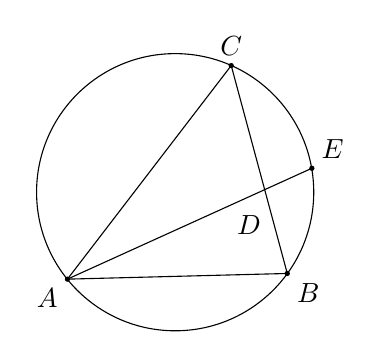
\begin{tikzpicture}[scale=0.8]
  \draw (0,0) circle (2.2);
  \coordinate (A) at (-1.71,-1.38);
  \coordinate (B) at (1.78,-1.29);
  \coordinate (C) at (0.89,2.01);
  \coordinate (E) at (2.17,0.38);
  \coordinate (D) at (1.42,0.04);
  \draw (A) -- (B) -- (C) -- cycle;
  \draw (A) -- (E);
  \fill (A) circle (1.2pt) node[below left] {$A$};
  \fill (B) circle (1.2pt) node[below right] {$B$};
  \fill (C) circle (1.2pt) node[above] {$C$};
  \fill (E) circle (1.2pt) node[above right] {$E$};
  \node at (1.17,-0.52) {$D$};
\end{tikzpicture}
\end{center}
\nopagebreak[4]
\Needspace{4\baselineskip}
\textbf{解析}
\nopagebreak[4]
\begin{center}% 1977 年黑龙江卷第 5 题：△ABC 内接于圆，∠A 的平分线 AE 交 BC 于 D、交外接圆于 E（按源卷布局）
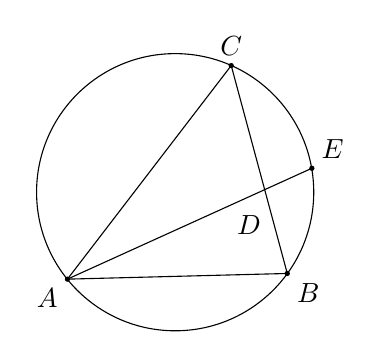
\begin{tikzpicture}[scale=0.8]
  \draw (0,0) circle (2.2);
  \coordinate (A) at (-1.71,-1.38);
  \coordinate (B) at (1.78,-1.29);
  \coordinate (C) at (0.89,2.01);
  \coordinate (E) at (2.17,0.38);
  \coordinate (D) at (1.42,0.04);
  \draw (A) -- (B) -- (C) -- cycle;
  \draw (A) -- (E);
  \fill (A) circle (1.2pt) node[below left] {$A$};
  \fill (B) circle (1.2pt) node[below right] {$B$};
  \fill (C) circle (1.2pt) node[above] {$C$};
  \fill (E) circle (1.2pt) node[above right] {$E$};
  \node at (1.17,-0.52) {$D$};
\end{tikzpicture}
\end{center}
\nopagebreak[4]
在 $\triangle ABD$ 与 $\triangle AEC$ 中找两组对应角相等。

\Needspace{5\baselineskip}
其一，$AD$ 平分 $\angle BAC$，而 $E$ 在射线 $AD$ 上，所以

\nopagebreak[4]
\[
\angle BAD=\angle DAC=\angle EAC.
\]

\Needspace{5\baselineskip}
其二，$D$ 在 $BC$ 上，故 $\angle ABD=\angle ABC$；$\angle ABC$ 与 $\angle AEC$ 都是弧 $AC$ 所对的圆周角，所以

\nopagebreak[4]
\[
\angle ABD=\angle AEC.
\]

\Needspace{5\baselineskip}
两角对应相等，得

\nopagebreak[4]
\[
\triangle ABD\sim\triangle AEC.
\]

\Needspace{5\baselineskip}
由相似比

\nopagebreak[4]
\[
\frac{AB}{AE}=\frac{AD}{AC},
\]

\Needspace{5\baselineskip}
即

\nopagebreak[4]
\[
AB\cdot AC=AD\cdot AE.
\]

\gkanswer{答案：见解析版}

\end{answer}
\begin{answer}
\gksolhead{6}{}

\textbf{题目}：

前进大队响应毛主席关于“绿化祖国”的伟大号召，1975 年造林 200 亩，又知 1975 年至 1977 年这三年内共造林 728 亩，求后两年造林面积的年平均增长率是多少？

\Needspace{4\baselineskip}
\textbf{解析}

\Needspace{5\baselineskip}
设后两年造林面积的年平均增长率为 $x$。则 1976 年造林 $200(1+x)$ 亩，1977 年造林 $200(1+x)^2$ 亩。三年共造林 728 亩：

\nopagebreak[4]
\[
200+200(1+x)+200(1+x)^2=728.
\]

\Needspace{5\baselineskip}
两边除以 200 并整理：

\nopagebreak[4]
\[
(1+x)^2+(1+x)-2.64=0.
\]

\Needspace{5\baselineskip}
解这个一元二次方程：

\nopagebreak[4]
\[
1+x=\frac{-1\pm\sqrt{1+4\times2.64}}{2}
=\frac{-1\pm\sqrt{11.56}}{2}
=\frac{-1\pm3.4}{2}.
\]

\Needspace{5\baselineskip}
取正根 $1+x=1.2$（负根 $-2.2$ 使 $1+x<0$，舍去），得

\nopagebreak[4]
\[
x=0.2=20\%.
\]

验算：$200+200\times1.2+200\times1.2^2=200+240+288=728$，符合题意。

\gkanswer{答案：$20\%$。}

\end{answer}
\begin{answer}
\gksolhead{7}{}

\textbf{题目}：

解方程：$\lg(2^x+2x-16)=x(1-\lg5)$。

\Needspace{4\baselineskip}
\textbf{解析}

\Needspace{5\baselineskip}
先化简右端。由 $1-\lg5=\lg10-\lg5=\lg2$，得

\nopagebreak[4]
\[
x(1-\lg5)=x\lg2=\lg2^x.
\]

\Needspace{5\baselineskip}
于是方程化为

\nopagebreak[4]
\[
\lg(2^x+2x-16)=\lg2^x.
\]

\Needspace{5\baselineskip}
对数相等且真数均为正，等价于真数相等：

\nopagebreak[4]
\[
2^x+2x-16=2^x
\quad\Longrightarrow\quad
2x=16
\quad\Longrightarrow\quad
x=8.
\]

验证：$x=8$ 时真数 $2^8+16-16=256>0$，且 $\lg256=8\lg2$，等式成立；又化简过程步步等价，故解唯一。

\gkanswer{答案：$x=8$。}

\end{answer}
\begin{answer}
\gksolhead{8}{}

\textbf{题目}：

已知三角形的三边成等差数列，周长为 $36\ \mathrm{cm}$，面积为 $54\ \mathrm{cm^2}$，求三边的长。

\begin{gktip}
\Needspace{0.25\textheight}
\textbf{附加题}
\end{gktip}

\textbf{附加题 9．（20 分）} 如图，$AP$ 表示发动机的连杆，$OA$ 表示它的曲柄。当 $A$ 在圆上作圆周运动时，$P$ 在 $x$ 轴上作直线运动，求 $P$ 点的横坐标。为什么当 $\alpha$ 是直角时，$\angle P$ 是最大？
\nopagebreak[4]
\begin{center}% 1977 年黑龙江卷附加题第 9 题：曲柄连杆机构，圆心 O、曲柄 OA（半径 R）、
% 连杆 AP（l）、曲柄转角 α 标在 O 处，P 在 x 轴上（按源卷布局）
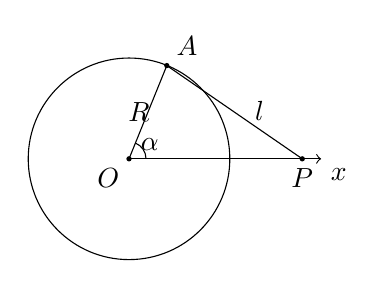
\begin{tikzpicture}[scale=0.8]
  \draw (0,0) circle (1.6);
  \coordinate (O) at (0,0);
  \coordinate (A) at (0.60,1.48);
  \coordinate (P) at (2.75,0);
  \draw[->] (0,0) -- (3.05,0) node[below right] {$x$};
  \draw (O) -- (A);
  \draw (A) -- (P);
  \draw (0.27,0) arc (0:68:0.27);
  \fill (O) circle (1.2pt) node[below left] {$O$};
  \fill (A) circle (1.2pt) node[above right] {$A$};
  \fill (P) circle (1.2pt) node[below] {$P$};
  \node at (0.16,0.75) {$R$};
  \node at (2.07,0.76) {$l$};
  \node at (0.33,0.22) {$\alpha$};
\end{tikzpicture}
\end{center}
\nopagebreak[4]
\textbf{参考题 10．} 求曲线 $y=\sin x$ 在 $[0,\pi]$ 上的曲边梯形绕 $x$ 轴旋转一周所形成的旋转体的体积。

\Needspace{4\baselineskip}
\textbf{解析}

\Needspace{5\baselineskip}
三边成等差数列，则中边是三边之和的算术平均，即 $\dfrac{36}{3}=12\ \mathrm{cm}$。设公差为 $d$，三边为

\nopagebreak[4]
\[
12-d,\qquad 12,\qquad 12+d.
\]

\Needspace{5\baselineskip}
半周长 $s=18$，由海伦公式：

\nopagebreak[4]
\[
S^2=18\bigl[18-(12-d)\bigr](18-12)\bigl[18-(12+d)\bigr]
=18(6+d)\times6\times(6-d)
=108(36-d^2).
\]

\Needspace{5\baselineskip}
由 $S=54$：

\nopagebreak[4]
\[
108(36-d^2)=54^2=2916
\quad\Longrightarrow\quad
36-d^2=27
\quad\Longrightarrow\quad
d^2=9
\quad\Longrightarrow\quad
d=3.
\]

三边长为 $9\ \mathrm{cm}$、$12\ \mathrm{cm}$、$15\ \mathrm{cm}$。

验算：$9+12+15=36$；又 $9^2+12^2=15^2$，是直角三角形，面积 $=\dfrac12\times9\times12=54\ \mathrm{cm^2}$，符合题意。

\textbf{附加题 9}
\nopagebreak[4]
\begin{center}% 1977 年黑龙江卷附加题第 9 题：曲柄连杆机构，圆心 O、曲柄 OA（半径 R）、
% 连杆 AP（l）、曲柄转角 α 标在 O 处，P 在 x 轴上（按源卷布局）
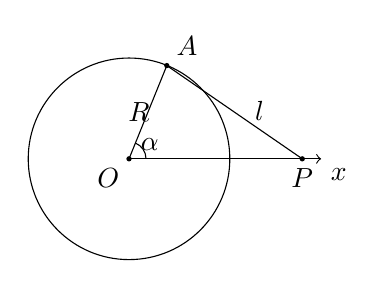
\begin{tikzpicture}[scale=0.8]
  \draw (0,0) circle (1.6);
  \coordinate (O) at (0,0);
  \coordinate (A) at (0.60,1.48);
  \coordinate (P) at (2.75,0);
  \draw[->] (0,0) -- (3.05,0) node[below right] {$x$};
  \draw (O) -- (A);
  \draw (A) -- (P);
  \draw (0.27,0) arc (0:68:0.27);
  \fill (O) circle (1.2pt) node[below left] {$O$};
  \fill (A) circle (1.2pt) node[above right] {$A$};
  \fill (P) circle (1.2pt) node[below] {$P$};
  \node at (0.16,0.75) {$R$};
  \node at (2.07,0.76) {$l$};
  \node at (0.33,0.22) {$\alpha$};
\end{tikzpicture}
\end{center}
\nopagebreak[4]
\Needspace{5\baselineskip}
设曲柄长 $OA=R$，连杆长 $AP=l$，以 $O$ 为原点、$x$ 轴沿 $OP$ 方向。设曲柄转角 $\alpha=\angle AOP$，则 $A$ 点坐标为

\nopagebreak[4]
\[
A=(R\cos\alpha,\ R\sin\alpha).
\]

\Needspace{5\baselineskip}
设 $P$ 点横坐标为 $x$（$P=(x,0)$），由连杆长度 $|AP|=l$：

\nopagebreak[4]
\[
(x-R\cos\alpha)^2+(0-R\sin\alpha)^2=l^2.
\]

\Needspace{5\baselineskip}
开方取正根（连杆伸向 $A$ 垂足的右侧）：

\nopagebreak[4]
\[
x=R\cos\alpha+\sqrt{l^2-R^2\sin^2\alpha}.
\]

这就是 $P$ 点的横坐标。

\Needspace{5\baselineskip}
再看 $\angle P$。设 $H$ 为 $A$ 在 $x$ 轴上的垂足，则 $\triangle AHP$ 为直角三角形，$\angle P$ 的对边 $AH=R\sin\alpha$，斜边 $AP=l$，于是

\nopagebreak[4]
\[
\sin\angle P=\frac{R\sin\alpha}{l}\le\frac{R}{l}.
\]

当 $\alpha=90^\circ$ 时 $\sin\alpha$ 取最大值 $1$，$\sin\angle P$ 达到最大 $\dfrac{R}{l}$；又 $0<\angle P<90^\circ$，正弦在该区间严格递增，所以此时 $\angle P$ 最大，即当 $\alpha$ 是直角时 $\angle P$ 最大。

\textbf{参考题 10}

\Needspace{5\baselineskip}
旋转体体积为曲边梯形绕 $x$ 轴旋转的积分：

\nopagebreak[4]
\[
V=\int_0^{\pi}\pi y^2\,dx
=\pi\int_0^{\pi}\sin^2x\,dx.
\]

\Needspace{5\baselineskip}
由 $\sin^2x=\dfrac{1-\cos2x}{2}$：

\nopagebreak[4]
\[
V=\pi\int_0^{\pi}\frac{1-\cos2x}{2}\,dx
=\pi\left[\frac{x}{2}-\frac{\sin2x}{4}\right]_0^{\pi}
=\pi\cdot\frac{\pi}{2}
=\frac{\pi^2}{2}.
\]

\gkanswer{答案：三边分别为 $9\ \mathrm{cm}$、$12\ \mathrm{cm}$、$15\ \mathrm{cm}$。}

\end{answer}